\documentclass[12pt]{jsarticle}
\usepackage[dvipdfmx]{graphicx}
\textheight = 25truecm
\textwidth = 18truecm
\topmargin = -1.5truecm
\oddsidemargin = -1truecm
\evensidemargin = -1truecm
\marginparwidth = -1truecm

\def\theenumii{\Alph{enumii}}
\def\theenumiii{\alph{enumiii}}
\def\labelenumi{(\theenumi)}
\def\labelenumiii{(\theenumiii)}
\def\theenumiv{\roman{enumiv}}
\def\labelenumiv{(\theenumiv)}
\usepackage{comment}
\usepackage{url}

%%%%%%%%%%%%%%%%%%%%%%%%%%%%%%%%%%%%%%%%%%%%%%%%%%%%%%%%%%%%%%%%
%% sty/ にある研究室独自のスタイルファイル
\usepackage{jtygm}  % フォントに関する余計な警告を消す
\usepackage{nutils} % insertfigure, figref, tabref マクロ

\def\figdir{./figs} % 図のディレクトリ
\def\figext{pdf}    % 図のファイルの拡張子

\begin{document}
%%%%%%%%%%%%%%%%%%%%%%%%%%%%
%% 表題
%%%%%%%%%%%%%%%%%%%%%%%%%%%%
\begin{center}
{\LARGE swimmyの機能追加の仕様書}
\end{center}

\begin{flushright}
  2021/4/1\\
  松田 陸斗
\end{flushright}
%%%%%%%%%%%%%%%%%%%%%%%%%%%%
%% 概要
%%%%%%%%%%%%%%%%%%%%%%%%%%%%
\section{はじめに}
\label{sec:introduction}

\section{追加した機能}
\label{sec:add_function}
\subsection{機能の概要}
本実験では,クイズを出題する機能を追加する.
クイズの取得には,OPEN TRIVIA DATABASE\cite{trivia}を利用する.
OPEN TRIVIA DATABASEとは,様々なクイズを提供しているWebAPIである.

また,追加した機能では,2通りの方法でクイズを出題することができる.
本実験で実装したクイズの出題方法を以下に示す.
\begin{enumerate}
  \item コマンドを入力した直後にクイズを出題する方法
  \item 指定した時刻にクイズを出題する方法
\end{enumerate}
ここで,追加した機能を呼び出すコマンドはtriviaである.
triviaコマンドは以下に示す引数を取ることができる.
% 追加した機能では,引数によって処理が分岐する.
% 本実験で実装した引数を以下に示す.
% また,追加した機能を呼び出すコマンドは\verb|trivia|である.
\begin{description}
  \item[trivia] すぐにクイズを出題する
  \item[trivia HH:MM] 毎日HH時MM分にクイズを出題する
  \item[trivia off] クイズの出題をやめる
  \item[trivia help] ヘルプを表示する
\end{description}

\subsection{機能の処理流れ}
追加した機能の処理流れを\figref{trivia_flow}に示す.
本機能の処理の開始は,Slackクライアントがコマンドを入力して呼び出す場合(以下,コマンド呼び出し)と,定期的に処理が繰り返される場合(以下,バッチ処理)がある.
また,\figref{trivia_flow}の処理流れの中にデータベース(以下,スケジュールDB)がある.
スケジュールDBは,クイズを通知する時刻とチャンネルを保存するデータベースである.
(実装では,データベースではなく,ハッシュを利用している.)
\figref{trivia_flow}の処理流れの説明を以下に示す.
\begin{description}
  \item[コマンド呼び出し]~
    \begin{enumerate}
      \item 引数があるか確認する
        \begin{enumerate}
          \item 引数がある場合
            \begin{enumerate}
              \item HH:MM\\
                コマンド呼び出し元のチャンネルと,引数で与えられた時刻(HH時MM分)をスケジュールDBに保存する
              \item off\\
                スケジュールDBに登録されているデータのうち,trivia offコマンドの呼び出し元チャンネルと一致するデータを削除する
              \item help\\
                triviaコマンドの引数一覧を取得する
              \item その他\\
                trivia helpコマンドを入力するように通知する
            \end{enumerate}
          \item 引数がない場合\\
            OPEN TRIVIA DATABASEからクイズを取得する
        \end{enumerate}
      \item クライアントに通知する
      \item コマンド終了\\
    \end{enumerate}
  \item[バッチ処理]~
    \begin{enumerate}
      \item 現在時刻を取得する
      \item スケジュールDBに登録されているすべてのデータを取得する
      \item 取得したデータのうち,現在時刻と一致するデータがあるか確認する
        \begin{enumerate}
          \item 一致するデータがある場合
            \begin{enumerate}
              \item 一致するデータの時刻を一日後の時刻に更新する
              \item OPEN TRIVIA DATABASEからクイズを取得する
              \item 一致するデータのチャンネルに通知する
              \item バッチ処理の開始に戻る
            \end{enumerate}
          \item 一致するデータがない場合\\
            バッチ処理の開始に戻る
        \end{enumerate}
    \end{enumerate}
\end{description}
\insertfigure[1.0]{trivia_flow}{trivia_flow}{追加した機能の処理流れ}

\subsection{機能の使用方法}
追加した機能は,Slack上でコマンドを入力して呼び出される.
追加した機能を呼び出す際の入力とswimmyの返信を以下に示す.
\begin{enumerate}
  \item trivia\\
    triviaコマンドの使用例とswimmyの返信を\figref{trivia}に示す.
  \item trivia HH:MM\\
    trivia HH:MMコマンドの使用例とswimmyの返信を\figref{trivia_HHMM}に示す.
  \item trivia off\\
    trivia offコマンドの使用例とswimmyの返信を\figref{trivia_off}に示す.
  \item trivia help\\
    trivia helpコマンドの使用例とswimmyの返信を\figref{trivia_help}に示す.
    % \begin{figure}[H]
    %   \centering
    %   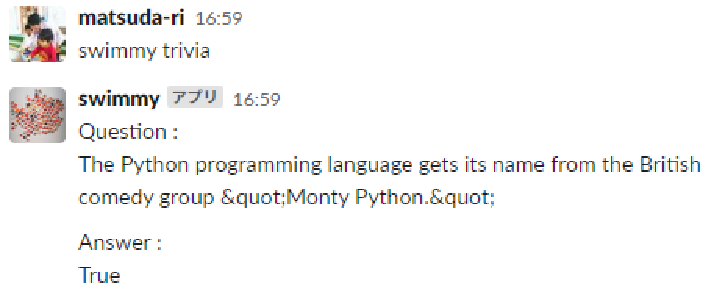
\includegraphics[scale=0.6]{figs/trivia.pdf}
    %   \caption{triviaコマンドの使用例とswimmyの返信}
    %   \label{fig:trivia}
    % \end{figure}
\end{enumerate}

\insertfigure[0.6]{trivia}{trivia}{triviaコマンドの使用例とswimmyの返信}

\insertfigure[0.6]{trivia_HHMM}{trivia_HHMM}{trivia HH:MMコマンドの使用例とswimmyの返信}

\insertfigure[0.6]{trivia_off}{trivia_off}{trivia offコマンドの使用例とswimmyの返信}

\insertfigure[0.6]{trivia_help}{trivia_help}{trivia helpコマンドの使用例とswimmyの返信}

\subsection{実装上の制限}
\begin{enumerate}
  \item 同じチャンネルに複数のスケジュールをセットできない(データベースでなく,ハッシュを使っているため)
  \item Botサーバが再起動するとスケジュールが消えてしまう(データベースでなく,ハッシュを使っているため)
\end{enumerate}

\section{おわりに}
\label{sec:conclusion}

% \appendix
% \section{付録}
%     \insertfigure[0.5]{trivia}{trivia}{triviaコマンドの使用例とswimmyの返信}

%     \insertfigure[0.5]{trivia_HHMM}{trivia_HHMM}{trivia HH:MMコマンドの使用例とswimmyの返信}

%     \insertfigure[0.5]{trivia_off}{trivia_off}{trivia offコマンドの使用例とswimmyの返信}

%     \insertfigure[0.5]{trivia_help}{trivia_help}{trivia helpコマンドの使用例とswimmyの返信}

\bibliographystyle{ipsjunsrt}
\bibliography{mybibdata}

\end{document}
